\documentclass[11pt, a4paper, oneside, UTF8]{ctexbook}
\usepackage{amsmath, amsthm, amssymb, bm, graphicx, hyperref, mathrsfs, enumitem, geometry, listings, xcolor, listings, fontspec, caption}

% 标题、作者、创建日期
\title{{\Huge{\textbf{PL/SQL学校课程笔记}}}\\ORACLE}
\author{徐鸣飞}
\date{2023年12月27日}

% 设置全局字体
\setmainfont{Times New Roman}   %设置英文正常字体为Times New Roman
\let\kaishu\relax %清除旧定义
\newCJKfontfamily\kaishu{KaiTi}[AutoFakeBold] %重定义\kaishu

% 设置页面的尺寸和布局。
\geometry{a4paper,scale=0.75}

% 行间距为1.5倍
\linespread{1.5}

% 定义定理环境
\newtheorem{theorem}{定理}[chapter]
\newtheorem{definition}[theorem]{定义}
\newtheorem{lemma}[theorem]{引理}
\newtheorem{corollary}[theorem]{推论}
\newtheorem{example}[theorem]{例}
\newtheorem{proposition}[theorem]{命题}

% 自定义配置
% 设置全局的 enumerate 环境项之间的距离
\setlist[enumerate]{itemsep=5pt, parsep=0pt, leftmargin=20pt, topsep=5pt, partopsep=0pt}
\setlist[itemize]{itemsep=5pt, parsep=0pt, leftmargin=20pt, topsep=5pt, partopsep=0pt}
% 定义新环境
% 定义颜色
\definecolor{commentcolor}{RGB}{182,73,1}
% 定义代码
\lstnewenvironment{java}[1][]{
  \lstset{
    language=Java,
    basicstyle=\ttfamily,
    keywordstyle=\color{blue},
    commentstyle=\color{green!60!black},
    stringstyle=\color{commentcolor},
    showstringspaces=false,
    breaklines=true,
    frame=single,
    flexiblecolumns=true,
    backgroundcolor=\color{gray!5},
    numbers=left,
    numberstyle=\tiny,
    #1
  }
}{}
\lstnewenvironment{plsql}[1][]{
  \lstset{
    language=SQL,
    morekeywords={BEGIN,DECLARE,END,IF,ELSE,ELSIF,LOOP,WHILE,PROCEDURE,FUNCTION},
    basicstyle=\ttfamily,
    keywordstyle=\color{blue},
    commentstyle=\color{green!60!black},
    stringstyle=\color{commentcolor},
    showstringspaces=false,
    breaklines=true,
    frame=single,
    flexiblecolumns=true,
    backgroundcolor=\color{gray!5},
    numbers=left,
    numberstyle=\tiny,
    #1
  }
}{}

% 文章开始
\begin{document}

% 生成标题
\maketitle

% 生成目录
\newpage                    %新的一页
\pagenumbering{Roman}       %页码以大写罗马数字形式表示
\setcounter{page}{1}        %设置当前页为第一页
\tableofcontents            %生成目录

% 生成内容
\newpage                    %新的一页
\pagenumbering{arabic}      %页码以阿拉伯数字形式表示
\setcounter{page}{1}        %设置当前页为第一页

% 文章内容
\chapter{导言}
\section{常见数据库}
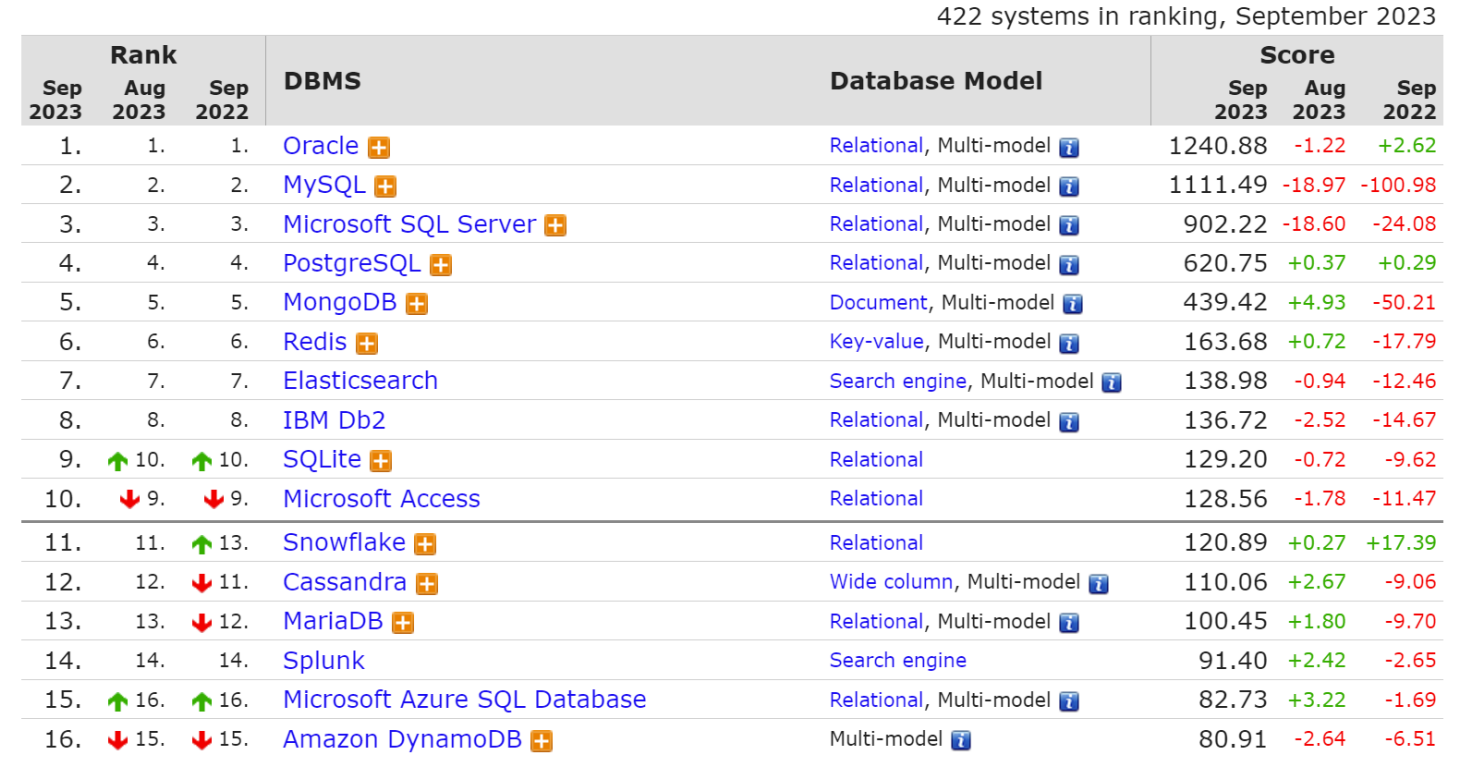
\includegraphics[width=0.9\linewidth]{picture/数据库占比对比.png}
\subsection{关系型数据库}
\subsubsection{MySQL}
MySQL是一款\textbf{开源的关系型数据库管理系统(RDBMS)},由瑞典MySQL AB公司开发,现由Oracle公司维护。以其轻量级、高效、快速的特性而闻名,适用于中小型应用和网站。MySQL支持多平台运行,包括Windows、Linux、macOS等,提供多种存储引擎如InnoDB、MyISAM等,具备良好的扩展性和广泛的社区支持。作为开源软件,MySQL允许用户免费获取、使用和修改其源代码,成为广泛应用于Web开发和其他应用场景的可靠数据库解决方案。
\subsubsection{Oracle}
Oracle是一款\textbf{商业性质的关系型数据库管理系统(RDBMS)},由Oracle公司开发。以其丰富的功能集、高级事务管理、安全性和卓越的性能而著称,适用于大型企业级应用。Oracle数据库支持复杂查询、分布式数据库、以及高并发环境下的大规模数据处理,具备出色的可伸缩性和性能优化特性。作为商业软件,Oracle提供了专业的技术支持、认证体系和咨询服务,成为众多大型组织和企业信赖的数据库解决方案。
\subsection{NoSQL数据库}
\subsubsection{文档型数据库:MongoDB}
\textbf{MongoDB是一种非关系型数据库管理系统(NoSQL DBMS),以其面向文档的存储模型而著称。}由MongoDB公司开发,采用分布式架构和灵活的模式设计,适用于处理大量非结构化或半结构化的数据。MongoDB的数据存储形式为BSON(Binary JSON),支持动态模式,使得数据存储和查询更加灵活。其强大的横向扩展性和自动分片功能使得MongoDB适用于大规模数据存储和处理,尤其在Web应用、大数据和实时分析等场景中表现出色。由于其开源特性,MongoDB拥有庞大的社区支持,为开发人员提供了丰富的资源和工具。
\subsubsection{搜索引擎:Elasticsearch}
\textbf{Elasticsearch是一种分布式数据库管理系统,专注于搜索和分析大规模数据。}作为开源软件,Elasticsearch构建在Apache Lucene之上,采用文档导向的存储模型,以JSON格式存储数据。其核心能力包括实时搜索、结构化查询和复杂分析,使其成为处理实时数据和日志、构建全文搜索引擎以及进行大规模数据分析的理想选择。通过支持分布式架构,Elasticsearch实现了水平扩展,能够应对高负载和大规模数据存储需求。该系统与Kibana等工具的整合形成了ELK堆栈,为用户提供了全面的数据管理、搜索和可视化解决方案。
\subsubsection{key-value数据库:redis}
\textbf{Redis是一款开源、高性能的键值对存储系统,属于NoSQL数据库的一种。}作为内存数据库,Redis将数据存储在内存中,提供了快速的读写访问速度,适用于对性能有严格要求的场景。其特色包括支持多种数据结构(如字符串、哈希表、列表、集合等),原子性操作,发布订阅机制等。虽然主要用于缓存、会话管理和实时数据分析等领域,但由于其快速响应和可持久化存储的能力,也在一些应用中用作主数据库。Redis的灵活性、简单性和高可用性,使其成为各种实时应用和分布式系统的理想选择。
\section{数据库发展趋势}
\subsection{1960s-1980s:层次数据库}
20世纪60年代到80年代的数据库技术被称为“层次结构”,也可以被称为网状结
构,无论标签是什么,这个时代的想法都旨在以树状结构组织数据结构。

\textbf{换而言之,这个时代的数据库技术是将数据存储为相互链接的记录。}
\begin{figure}[htbp]
  \center
  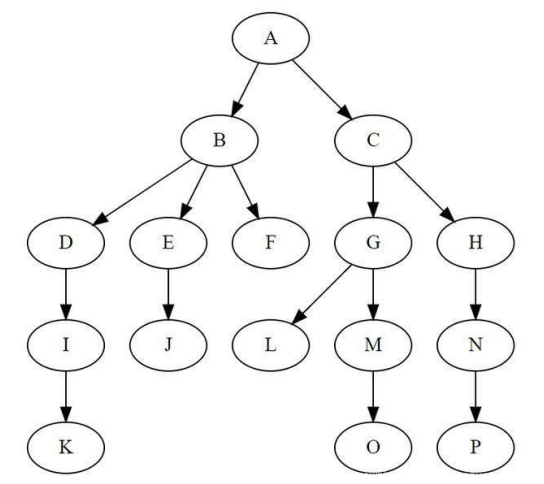
\includegraphics[width=0.5\textwidth]{picture/层次数据库示意图.png}
  \caption{层次数据库示意图}
  \label{fig:hierarchicalDatabase}
\end{figure}
在层次数据库的模型中,数据以节点的形式存在,每个节点可以包含一个或多个字段,形成父子关系。根节点是顶层节点,而叶节点是没有子节点的底层节点。层次数据库适用于需要表示层次结构信息的场景,如组织结构、文件系统等。尽管在过去曾经流行,但由于关系型数据库的普及,层次数据库在现代数据库系统中的应用相对较少。其特点包括数据重复、路径的唯一性以及专门的查询语言用于数据检索和更新。
\subsection{1980s-2000s:实体关系数据库}
实体关系数据库(Entity-Relationship Database)是一种基于实体-关系模型的数据库系统,用于存储和管理数据。在这个模型中,数据以实体(Entity)和实体之间的关系(Relationship)为核心。每个实体都有属性,而实体之间的关系描述了这些实体之间的联系和交互。

实体关系数据库的优势在于其规范化的数据结构、ACID 特性(原子性、一致性、隔离性、持久性)以及使用 SQL(Structured Query Language)进行数据操作和查询的能力。这种数据库模型在处理复杂的关联数据和支持事务处理方面表现出色,因此在各种应用场景中广泛应用,包括企业应用、金融系统、医疗信息管理等。

关系型数据库采用了关系代数的概念,数据以表格(表)的形式组织,每个表表示一个实体,表中的行代表实体的具体实例,而列代表实体的属性。实体之间的关系则通过外键来建立。
\begin{figure}[htbp]
  \center
  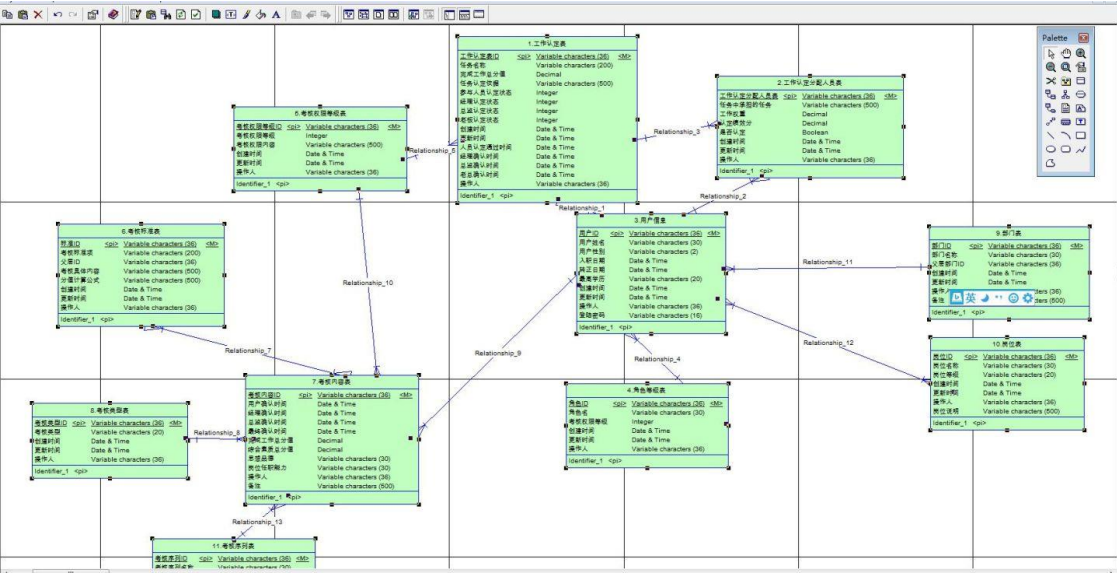
\includegraphics[width=0.5\textwidth]{picture/实体关系数据库示意图.png}
  \caption{实体关系数据库示意图}
  \label{fig:relationDatabase}
\end{figure}
\subsection{2000s-2020s:NoSQL}
NoSQL为Not Only SQL的缩写,是对不同于传统的关系型数据库的数据库管理系统的统称。

\textbf{网络上的数据本质上不是表格的结构。}

NoSQL常用于超大规模数据的存储(例如谷歌或Facebook每天为他们的用户收集万亿比特的数据)。这些类型的数据存储不需要固定的模式,无需多余操作就可以横向扩展。

\begin{center}
  \begin{minipage}{\textwidth}
    \center
    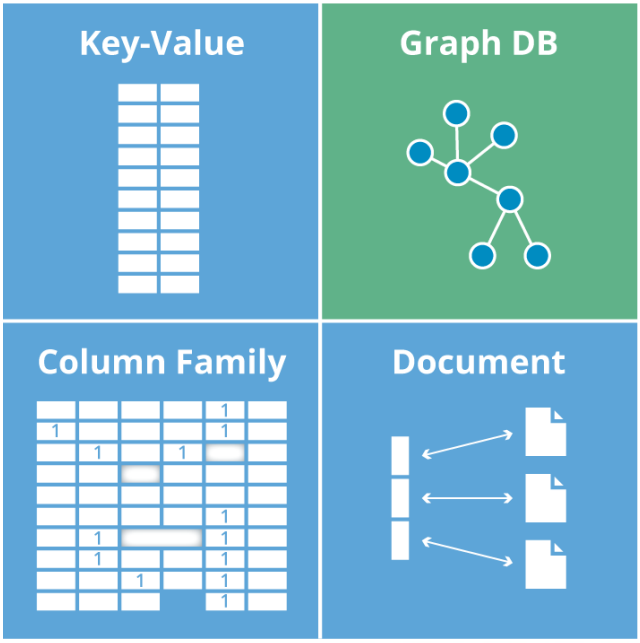
\includegraphics[width=0.5\textwidth]{picture/NoSQL数据库示意图.png}
    \captionsetup{hypcap=false}
    \captionof{figure}{NoSQL数据库示意图}
    \label{fig:NosqlDatabase}
  \end{minipage}
\end{center}

\subsection{2020s-未知:图数据库}
这个创新时代正在从存储系统的效率转向\textbf{从存储系统包含的数据中提取价值}。

\textit{即价值从效率转移到高度连接的数据资产中衍生。}

\section{SQL*Plus工具}
\subsection{介绍}
SQLPlus是Oracle数据库系统中的一种交互式查询工具和脚本处理器。它是一个{\bfseries\kaishu 命令行工具},允许用户连接到Oracle数据库并执行SQL查询、PL/SQL块以及其他数据库管理任务。

\subsection{交互过程}
\begin{center}
  \begin{minipage}{\textwidth}
    \center
    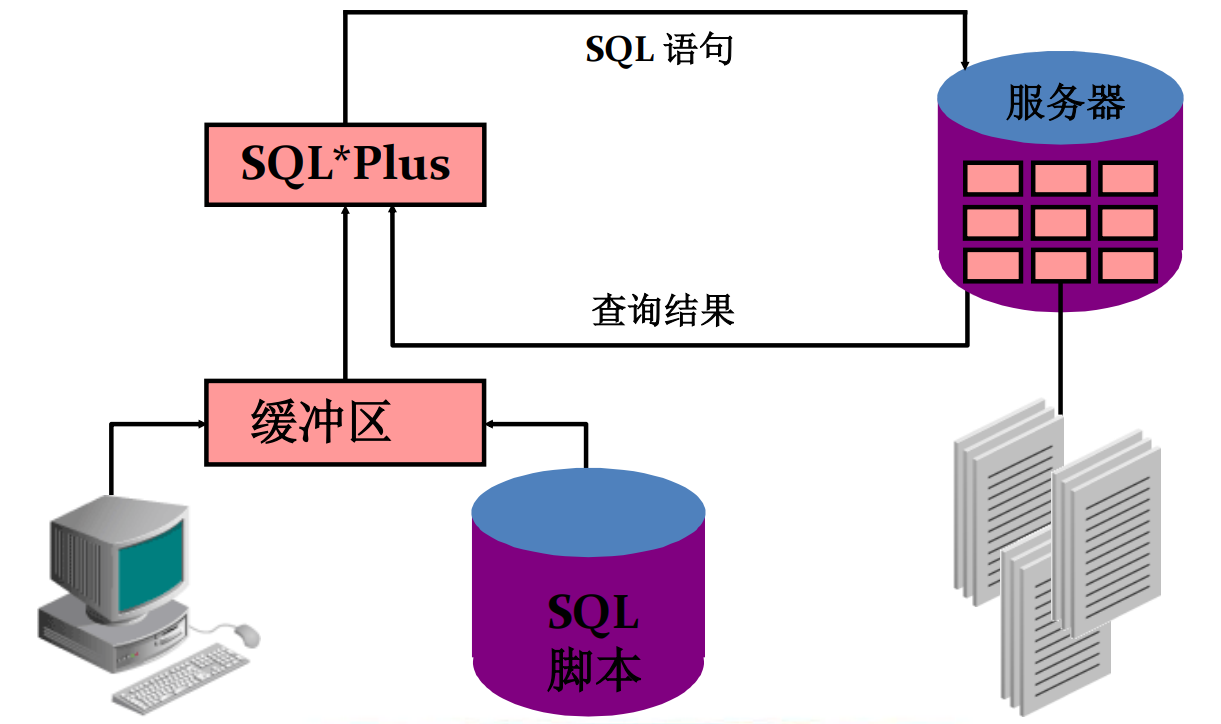
\includegraphics[width=0.7\textwidth]{picture/SQLPLUS交互.png}
    \captionsetup{hypcap=false}
    \captionof{figure}{SQL*Plus交互示意图}
    \label{fig:SQLPLUS交互}
  \end{minipage}
\end{center}
参与组件介绍:
\begin{description}
  \item[用户界面] 用户与SQLPlus进行交互的地方,可以是命令行界面或其他支持SQLPlus的用户界面。用户通过这个界面输入SQL查询、PL/SQL块或SQL*Plus命令。
  \item[SQL*Plus引擎] SQLPlus引擎是一个解释器,负责解释和执行用户输入的SQLPlus命令,以及管理与Oracle数据库的交互。它解析并执行SQL查询、PL/SQL块,处理输出格式,管理连接和会话等。
  \item[OCI(Oracle Call Interface)] OCI是Oracle数据库提供的一组API(应用程序接口),允许应用程序(包括SQLPlus)与Oracle数据库进行通信。\textbf{SQLPlus使用OCI}与数据库建立连接、发送SQL命令,以及接收执行结果。
  \item[Oracle数据库引擎] 这是实际执行SQL查询、PL/SQL块的地方。当SQLPlus将命令发送给数据库时,Oracle数据库引擎负责解析和执行这些命令,然后返回结果给SQLPlus。
  \item[数据缓冲区] SQL*Plus通常会在本地维护一个数据缓冲区,用于存储从数据库检索到的数据。这使得用户可以在本地对结果进行分析、浏览和编辑。
\end{description}
\subsection{Oracle数据库连接命令}
在CMD中运行SQLPlus并连接到Oracle服务器的命令为:

{\bfseries\kaishu sqlplus <用户名>/<密码>@//<数据库IP>:<Port>/<服务名>}

如:
\begin{example}
  sqlplus system/system@//192.168.146.132:1521/helowin
\end{example}

\subsection{常用编辑命令}
\begin{description}
  \item[DESC] DESCRIBE,显示表结构,包括表的列名、数据类型和约束信息,效果见图\ref{fig:DESC_SQLPLUS}。
  \item[L] 列出当前缓冲区中的 SQL 语句(未执行)的命令。
    \item[\textup{[N]}] number,选中第n行;[n]后可追加内容[text]来替换第n行或新建第n行。
  \item[A] APPEND,追加文本到缓冲区中的当前选中行。使用“.”单独一行表示结束追加。使用前要求缓冲区内存在文本。
  \item[C] CHANGE,修改缓冲区中的当前选中行的文本,格式为{\bfseries\kaishu C /<原文>/<新文>}。
  \item[DEL] DELETE,删除缓冲区中的当前选中行。可追加[n]代表删除第n行;追加[n][m]删除第n至m行。
  \item[$\boldsymbol{/}$] 运行在SQL缓冲区中的SQL语句。
  \item[CL] CLEAR,清除 SQL*Plus 屏幕上的内容,将屏幕滚动条移至顶部。
\end{description}
\begin{figure}[htbp]
  \center
  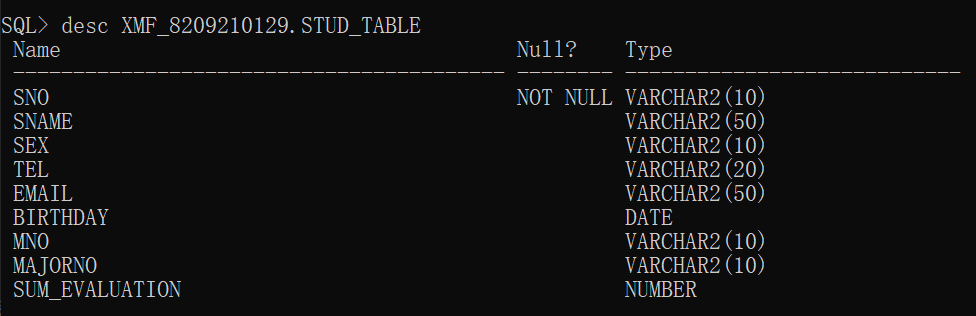
\includegraphics[width=\textwidth]{picture/DESC_SQLPLUS效果.png}
  \caption{DESC效果图}
  \label{fig:DESC_SQLPLUS}
\end{figure}

使用编辑缓冲区的命令前,需保证缓存区中存在内容:

\begin{center}
  \begin{minipage}{\textwidth}
    \center
    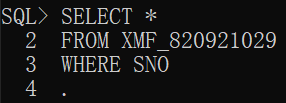
\includegraphics[width=0.5\textwidth]{picture/输入内容到缓冲区.png}
    \captionsetup{hypcap=false}
    \captionof{figure}{输入内容到缓冲区,使用enter换行,使用单独的.结束}
    \label{fig:输入内容到缓冲区}
  \end{minipage}
\end{center}

可使用L查看缓冲区:

\begin{center}
  \begin{minipage}{\textwidth}
    \center
    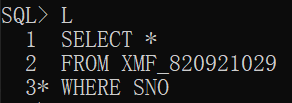
\includegraphics[width=0.5\textwidth]{picture/L命令效果.png}
    \captionsetup{hypcap=false}
    \captionof{figure}{L命令效果图}
    \label{fig:L命令效果}
  \end{minipage}
\end{center}

*号所在行为正在编辑行。
可使用数字更改选中行后,使用A命令添加内容:

\begin{center}
  \begin{minipage}{\textwidth}
    \center
    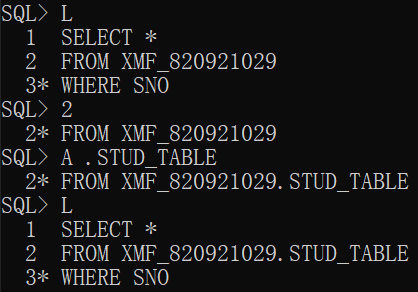
\includegraphics[width=0.5\textwidth]{picture/A命令效果.png}
    \captionsetup{hypcap=false}
    \captionof{figure}{A命令、n命令效果图}
    \label{fig:A命令效果}
  \end{minipage}
\end{center}

可使用C命令更改指定行(注意原文与新文中无空格):

\begin{center}
  \begin{minipage}{\textwidth}
    \center
    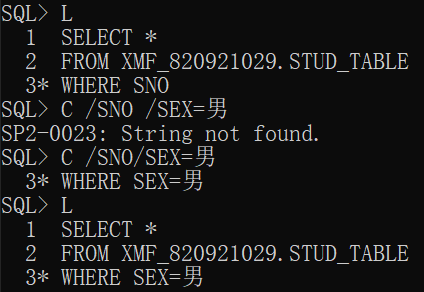
\includegraphics[width=0.5\textwidth]{picture/C命令效果.png}
    \captionsetup{hypcap=false}
    \captionof{figure}{C命令效果图}
    \label{fig:C命令效果}
  \end{minipage}
\end{center}

可使用DEL命令删除指定行:

\begin{center}
  \begin{minipage}{\textwidth}
    \center
    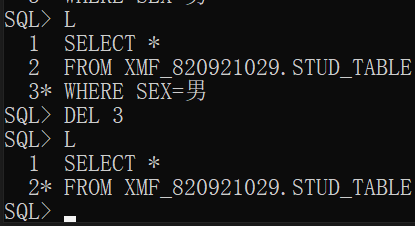
\includegraphics[width=0.5\textwidth]{picture/DEL命令效果.png}
    \captionsetup{hypcap=false}
    \captionof{figure}{DEL命令效果图}
    \label{fig:DEL命令效果}
  \end{minipage}
\end{center}

再次使用n命令新建行:

\begin{center}
  \begin{minipage}{\textwidth}
    \center
    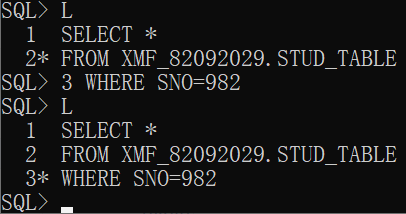
\includegraphics[width=0.5\textwidth]{picture/N命令效果图.png}
    \captionsetup{hypcap=false}
    \captionof{figure}{N命令效果图}
    \label{fig:N命令效果}
  \end{minipage}
\end{center}

使用$\boldsymbol{/}$运行(使用后缓冲区不会被清除):

\begin{center}
  \begin{minipage}{\textwidth}
    \center
    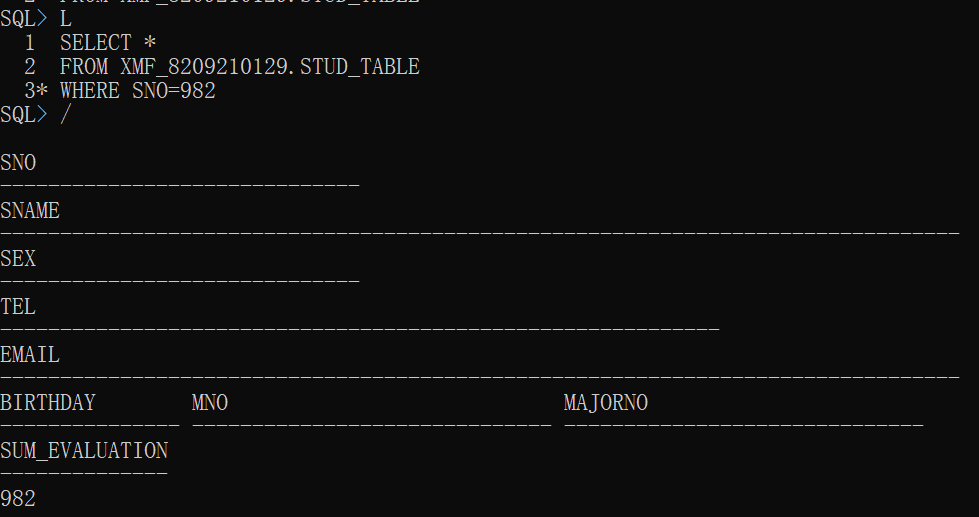
\includegraphics[width=0.5\textwidth]{picture/运行命令效果图.png}
    \captionsetup{hypcap=false}
    \captionof{figure}{运行命令效果图}
    \label{fig:运行命令效果}
  \end{minipage}
\end{center}

\subsection{SQL文件存取命令}

\begin{description}
  \item[SAVE] 把SQL缓冲区的内容存入指定的文件,如 \textit{SAVE D:\textbackslash SQL\textbackslash SMAPLE}。
  \item[GET] 将指定的脚本文件装入SQL缓存区,如\textit{GET D:\textbackslash SQL\textbackslash SMAPLE}。
  \item[START] @ 或START,把指定的脚本文件装入SQL缓冲区并运行,如\textit{@ D:\textbackslash SQL\textbackslash SMAPLE.sql}。
\end{description}

\subsection{输出保存命令}
SPOOL,语法为:\\
{\bfseries\kaishu SPO[OL] [File\_name[.ext]] [[CRE[ATE]|REP[LACE]|APP[END]] | OFF | OUT ]}。

参数说明:
\begin{description}
  \item[File\_name] 指定脱机文件的名称,默认的文件扩展名为LST。
    \item[\textup{CRE[ATE]}] 表示创建一个新的脱机文件,这也是SPOOL命令的默认状态。
    \item[\textup{REP[LACE]}] 表示替代已经存在的脱机文件。
    \item[\textup{APP[END]}] 表示把脱机内容附加到一个已经存在的脱机文件中。
  \item[OFF | OUT] 表示关闭SPOOL输出。
\end{description}

\chapter{PL/SQL语法学习}
\section{PL/SQL概述}
\subsection{介绍}
\textbf{PL/SQL(Procedural Language/Structured Query Language)}:一种\textbf{过程化编程语言},专门用于\textbf{Oracle数据库系统}。它将SQL(Structured Query Language)语句与结构化程序设计语言(如条件、循环等)相结合,提供了一种强大的方式来处理和操作数据库中的数据。

\subsection{优点}
\begin{enumerate}
  \item {\bfseries\kaishu 数据库集成:} PL/SQL是为数据库设计的,能够直接嵌套在SQL中;许多与数据库有关的应用程序功能都已经集成在PL/SQL语言中。
  \item {\bfseries\kaishu 模块化开发:} PL/SQL允许将代码模块化组织,通过存储过程和包的方式来管理和封装代码。这有助于提高代码的可维护性和重用性。
  \item {\bfseries\kaishu 性能优化:}PL/SQL支持存储过程和函数,可以在数据库中预编译和存储,提高了执行效率。此外,PL/SQL还支持游标,能够有效地处理大量的数据。
\end{enumerate}
此外,还有其他如\textbf{安全性}(PL/SQL能够帮助限制对数据库的直接访问,从而提高了数据库的安全性)、\textbf{灵活性}(PL/SQL具有丰富的控制结构和数据类型,使其既可以用于简单的SQL查询,也可以用于复杂的业务逻辑实现)、\textbf{事务控制}( PL/SQL提供了强大的事务控制功能,支持原子性、一致性、隔离性和持久性(ACID属性),确保了数据库操作的可靠性和一致性)等优点。

\subsection{执行体系}
\begin{center}
  \begin{minipage}{\textwidth}
    \center
    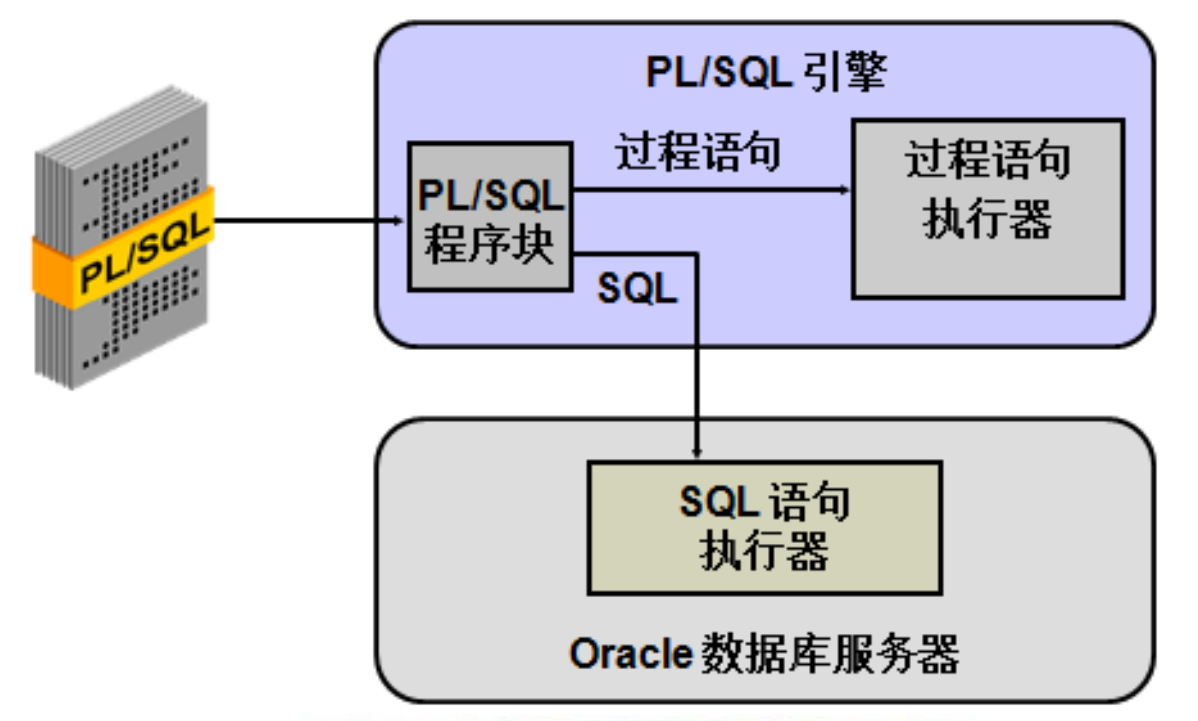
\includegraphics[width=0.5\textwidth]{picture/PLSQL执行体系.png}
    \captionsetup{hypcap=false}
    \captionof{figure}{PLSQL执行体系示意图}
    \label{fig:PLSQL执行体系}
  \end{minipage}
\end{center}
从图\ref{fig:PLSQL执行体系}中这些组件的角度来看PL/SQL的执行过程:
\begin{description}
  \item[PL/SQL引擎] \hfill
    \begin{itemize}
      \item PL/SQL解释器: 编译后的PL/SQL代码由PL/SQL引擎的解释器执行。解释器负责逐行执行PL/SQL代码,并管理变量、控制流程、处理异常等。
      \item 数据交互: 在PL/SQL执行过程中,可能涉及到与数据库的交互,例如执行SQL语句、操作数据等。这些交互通过PL/SQL引擎协调实现。
    \end{itemize}
  \item[过程语句执行器] \hfill
    \begin{itemize}
      \item 过程语句解析: 如果PL/SQL程序包含了过程性语句,这些语句将被PL/SQL引擎的过程语句执行器处理。这可能包括存储过程、函数或触发器的调用。
      \item 编译过程性代码: 过程语句执行器会编译PL/SQL代码,将其转换为可执行的形式。这个编译过程包括语法检查、编译成中间代码等步骤。
    \end{itemize}
  \item[SQL执行器]  \hfill
    \begin{itemize}
      \item 接收SQL语句: 当一个包含PL/SQL代码的程序被触发时,其中可能包含SQL语句。这些SQL语句被传递给SQL执行器,它负责执行这些语句。
      \item 解析SQL语句: SQL执行器解析SQL语句,进行语法分析和语义检查。在这个阶段,执行计划被生成,这是一个描述如何执行查询的内部表示。
    \end{itemize}
  \item[Oracle数据库服务器] \hfill
    \begin{itemize}
      \item 数据存储和检索: 当PL/SQL程序执行SQL语句时,Oracle数据库服务器负责实际的数据存储和检索。执行计划告诉数据库服务器如何最有效地执行查询,并从表中检索或修改数据。
    \end{itemize}
\end{description}

当有过程调用或SQL语句执行时,流程可能涉及多次从PL/SQL引擎到SQL执行器,再到数据库服务器的交互。

需要注意的是,Oracle数据库的内部执行细节是复杂的,并且可能受到优化、缓存、并发控制等多方面的影响。

\section{程序块结构}
PL/SQL程序块是PL/SQL语言中的基本结构,它可以包含变量、常量、游标、异常处理等元素。PL/SQL程序块有三种主要形式:匿名块、存储过程和存储函数。
类型说明:
\begin{enumerate}
  \item {\bfseries\kaishu 匿名块(Anonymous blocks)}:没有命名的程序块。匿名块是在应用程序内部需要的地方声明的,在这个应用程序每次执行时,这些匿名块都会被编译并执行。
  \item  {\bfseries\kaishu 过程(Procedures)}和{\bfseries\kaishu 函数 (Functions) }:过程和函数也统称为\textit{子程序 (Subprograms)},子程序是对匿名块的补充,子程序就是被命名的PL/SQL程序块,而它们可以存储在数据库中。
\end{enumerate}
一个简单的PL/SQL匿名块的结构如下:
\begin{plsql}[caption=PL/SQL匿名块示例代码]
DECLARE
  -- 声明变量和常量
  variable_name datatype;
  constant_name CONSTANT datatype := value;

BEGIN
  -- 可执行的PL/SQL代码
  -- 可以包括各种语句,如赋值、条件语句、循环等
  -- 例如:
  variable_name := value;
  IF condition THEN
  -- do something
  END IF;

EXCEPTION
  -- 异常处理部分
  -- 处理可能出现的异常
  -- 例如:
  WHEN others THEN
  -- handle exception

END;
/
\end{plsql}
一个简单的PL/SQL函数的示例代码(获取员工薪水):
\begin{plsql}[caption=获取员工薪水函数示例代码]
CREATE OR REPLACE FUNCTION get_employee_salary(p_employee_id NUMBER)
  RETURN NUMBER
  IS
  -- 声明变量
  v_salary NUMBER;
BEGIN
  -- 查询员工薪水
  SELECT salary INTO v_salary
  FROM employees
  WHERE employee_id = p_employee_id;

  -- 返回薪水
  RETURN v_salary;
END;
/
\end{plsql}
一个简单的PL/SQL过程的示例代码(更新员工薪水):
\begin{plsql}[caption=更新员工薪水过程示例代码]
CREATE OR REPLACE PROCEDURE update_employee_salary(p_employee_id NUMBER, p_new_salary NUMBER)
  IS
BEGIN
  -- 更新员工薪水
  UPDATE employees
  SET salary = p_new_salary
  WHERE employee_id = p_employee_id;

  -- 提交事务
  COMMIT;
END;
/
\end{plsql}
程序块结构说明:
\begin{description}
  \item[DECLARE] {\bfseries\kaishu 可选},\textit{声明段},以关键字DECLARE开始并以执行段的开始而结束。
  \item[BEGIN] {\bfseries\kaishu 必选},\textit{执行段},以关键字BEGIN开始而以关键字END或关键字EXCEPTION结束。
  \item[EXCEPTION] {\bfseries\kaishu 可选},\textit{异常处理段},以关键字EXCEPTION开始,以关键字END结束。
\end{description}
执行规则:
\begin{enumerate}
  \item 每一个PL/SQL控制语句都是以分号(;)结束。
  \item 使用正斜杠(/)运行SQL*Plus内存缓冲区的匿名PL/SQL程序块。
\end{enumerate}

\section{变量}
 {\bfseries\kaishu 变量},就是内存中一个命名的临时存储区,而变量中所存储的信息就是这个变量的当前值。

在PL/SQL中,在使用一个变量之前,必须首先声明这个变量。一旦声明了这个变量,就可以在SQL语句和过程化(PL/SQL)语句中使用这个变量了。

变量使用步骤:
\begin{enumerate}
  \item 在声明部分(DECLARE块)\textbf{声明和初始化}变量
  \item 在执行部分(BEGIN块)为变量\textbf{赋新值}
  \item 通过参数将值传入PL/SQL块
  \item 通过输出变量来查看结构
\end{enumerate}
\subsection{变量命名规则}
\begin{itemize}
  \item 必须{\bfseries\kaishu 以英语字母开始}
  \item 可以包含{\bfseries\kaishu 英语字母}或{\bfseries\kaishu 数字}或{\bfseries\kaishu 特殊字符}——美元号(\$)、下划线(\_)、和井号(\#)
  \item 长度最长为{\bfseries\kaishu 30}个字符
  \item {\bfseries\kaishu 不区分大小写}
  \item 不能是保留关键字
  \item 不能与数据库的表或列同名
\end{itemize}
\subsection{变量声明语法}
在引用PL/SQL程序块中的变量之前,必须在声明段声明所有的变量(标识符)。
在声明变量的同时还可以为变量赋初值,但是在声明变量时赋予初始值是可选的。
如果在一个变量声明中引用了其他变量,一定要确保在之前的语句中已经声明了引用的变量。

声明语法:
{\bfseries\kaishu 标识符 [CONSTANT] 数据类型 [NOT NULL] [:= initial\_value]}

\begin{plsql}[caption=PL/SQL变量声明语法示例]
  DECLARE
  v_dogid NUMBER(10) NOT NULL := 38;
  v_name VARCHAR2(25) := ‘White Tiger’
  c_color CONSTANT VARCHAR2(15) := ‘White’
  v_birthday DATE;
\end{plsql}

\subsection{变量类型}
PL/SQL支持四大类数据类型(最常用的是标量数据类型,目前熟悉这个即可):
\begin{enumerate}
  \item 标量(Scalar)数据类型:
        \begin{itemize}
          \item NUMBER: 用于存储数值,可以是整数或小数。
                \begin{itemize}
                  \item NUMBER(p,s):数据型数据,p 表示精度(总位数),s 表示小数部分的位数
                  \item BINARY\_INTEGER:基本整型数
                  \item PLS\_INTEGER:基本带符号整数型
                  \item BINARY\_FLOAT:存储单精度浮点数,以IEEE754格式表示浮点数,它需要5个字节来存储数字
                  \item BINARY\_DOUBLE:存储双精度浮点数,以IEEE754格式表示浮点数,它需要9个字节来存储数字
                \end{itemize}
          \item character: 字符型数据类型,用于存储字符串。
                \begin{itemize}
                  \item VARCHAR2(size):基本变长字符型数据
                  \item CHAR(size):基本定长字符型数据
                \end{itemize}
          \item DATE: 用于存储日期和时间。
                \begin{itemize}
                  \item DATA:基本日期和时间数据
                  \item TIMESATMP(precision):该数据类型除了日期和时间之外还包括了多达小数点后9位秒数
                \end{itemize}
          \item BOOLEAN: 用于存储布尔值(TRUE 或 FALSE)。
                \begin{itemize}
                  \item BOOLEAN:基本逻辑类型,它只能存储逻辑计算的3个可能值之一
                \end{itemize}
        \end{itemize}
  \item 组合(Composite)数据类型:
        \begin{itemize}
          \item \%ROWTYPE: 表示一个表行的结构,通常在变量声明中使用。
          \item RECORD: 类似于\%ROWTYPE,但可以自定义结构。
          \item TABLE: 用于存储同一数据类型的集合。可以是索引表(INDEX BY)或关联数组。
        \end{itemize}
  \item 引用(Reference)数据类型:
        \begin{itemize}
          \item REF CURSOR: 用于存储游标引用,可用于动态查询结果的处理。
          \item PL/SQL RECORD: 通过 TYPE 语句定义的记录类型。
        \end{itemize}
  \item 大对象(LOB)数据类型:
        \begin{itemize}
          \item CLOB (Character Large Object): 用于存储大量字符数据,如文本。
          \item BLOB (Binary Large Object): 用于存储二进制数据,如图像、音频等。
          \item NCLOB (National Character Large Object): 类似于 CLOB,但用于存储国家字符集数据。
          \item BFILE: 用于存储二进制文件的地址引用,文件存储在数据库外部。
        \end{itemize}
\end{enumerate}
\subsection{变量声明建议}
\begin{enumerate}
  \item 遵守命名的规则,变量的命名规则与SQL对象的命名规则完全相同。
  \item 必须初始化被指定为非空(NOT NULL)和常量(Constant)的变量。
  \item 一行最好只声明一个标识符以提高代码的易读性和方便代码的维护。
  \item 通过使用赋值操作符(:=)或默认关键字(DEFAULT)来初始化标识符。
  \item 变量最好不要与列名重名。
  \item 两个PL/SQL变量(对象)只要在不同的程序块中是可以同名的。
  \item 如果没有必要就不要在PL/SQL变量上强加非空(NOT NULL)约束。
  \item 代码中使用了 PL/SQL 游标、BLOB/CLOB Locator 或其他需要手动释放的资源,请确保在不再需要它们时及时释放这些资源,以避免内存泄漏。
\end{enumerate}
\subsection{赋值:字符串分隔符(引号限定符)}
\subsubsection{介绍}
q 和 p 是引号限定符,用于创建带有引号的字符串字面量。具体而言,q 和 p 用于创建带有引号的标识符或字符串,这样可以在字符串中包含特殊字符,而不必使用转义字符。q 用于创建带有双引号的标识符,而 p 用于创建带有单引号的字符串。

(注意:p 定界符可以使用大多数字符作为定界符,但不能使用双引号 ",单引号 ',反引号 `,右括号 ),右中括号 ],右大括号 \} 和感叹号 ! 作为定界符。)
\subsubsection{演示}
不使用字符串分隔符的情况:
\begin{plsql}[caption=不使用字符串分隔符]
DECLARE
  v_message VARCHAR2(100);
BEGIN
  -- 使用双单引号进行转义
  v_message := 'He said, ''Hello World!''';

  -- 打印字符串
  DBMS_OUTPUT.PUT_LINE(v_message);
END;
\end{plsql}
使用字符串分隔符后:
\begin{plsql}[caption=使用字符串分隔符]
DECLARE
  v_message VARCHAR2(100);
BEGIN
  -- 使用 q'...' 创建原始字符串
  v_message := q'{He said, 'Hello World!'}';

  -- 打印字符串
  DBMS_OUTPUT.PUT_LINE(v_message);
END;
\end{plsql}
\begin{center}
  \begin{minipage}{\textwidth}
    \center
    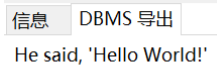
\includegraphics[width=0.3\textwidth]{picture/字符串分隔符效果图.png}
    \captionsetup{hypcap=false}
    \captionof{figure}{字符串分隔符输出演示}
    \label{fig:字符串分隔符效果图}
  \end{minipage}
\end{center}
\subsection{类型声明:\%TYPE属性}
为了避免这种变量数据类型和精度的硬编码(即数据类型和精度必须显式定义),PL/SQL引入\%TYPE属性。程序员(开发人员)可以使用\%TYPE属性按照之前已经声明过的变量或数据库的列来声明一个变量。当存储在一个变量中值来自于数据库中的表时,使用\%TYPE属性来声明这个变量时再适合不过的了。

\subsubsection{使用语法}
\begin{enumerate}
  \item 标识符 表名.列名\%TYPE
  \item 标识符 定义好的变量\%TYPE
\end{enumerate}
\subsubsection{案例}
\begin{plsql}
DECLARE
  v_data emp.data%TYPE
  v_Month_Value NUMBER(6,4) := 3.25
  v_Year_Value v_Month_Value%TYPE := 4.40
\end{plsql}
好处:
\begin{enumerate}
  \item 可以不知道emp表中的data列或v\_Month\_Value的数据类型和精度就直接使用对应类型。
  \item 当emp的data列或者v\_Month\_Value的数据类型和精度发生变化时,v\_data和v\_Year\_Value也会随之变化。
\end{enumerate}
\section{布尔变量与布尔表达式}
布尔变量和布尔表达式在任何程序语言设计上都是非常重要和广泛使用的。在PL/SQL程序中,可以在SQL语句中也可以在过程化语句中进行变量的比较,这样的比较表达式被称为布尔表达式,它们是由单个表达式或由关系操作符所分隔的复杂表达式所组成。

特性:
\begin{itemize}
  \item 只有{\bfseries\kaishu 值TURE、FALSE和NULL}可以赋给一个布尔变量。
  \item 可以通过{\bfseries\kaishu 逻辑操作符AND、OR和NOT}对布尔变量进行运算,运算总是产生TURE、FALSE或NULL。
  \item 数字、字符和日期表达式可以被用来返回一个布尔值。
\end{itemize}
\subsection{布尔操作符}
\begin{center}
  \begin{minipage}{\textwidth}
    \center
    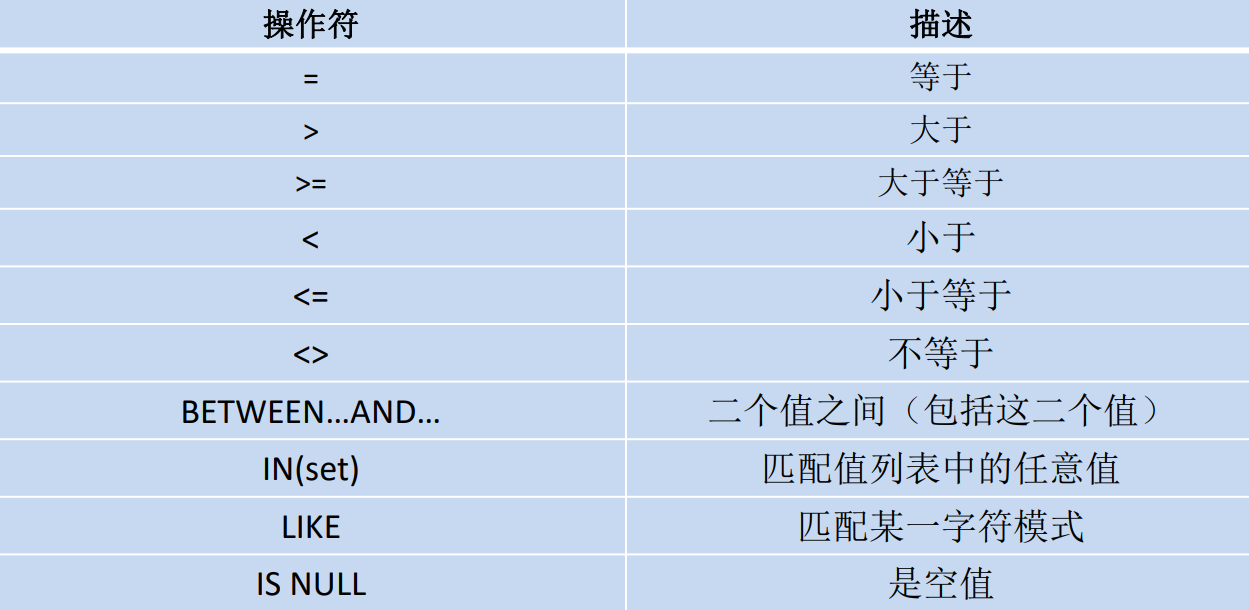
\includegraphics[width=\textwidth]{picture/布尔操作符.png}
    \captionsetup{hypcap=false}
    \captionof{figure}{布尔操作符}
    \label{fig:布尔操作符}
  \end{minipage}
\end{center}
\section{代替变量和绑定变量}
\subsection{代替变量}
因为PL/SQL本身没有输入和输出功能,所以必须依赖于执行PL/SQL程序的环境变量值传入或传出PL/SQL程序块。

在SQL*Plus环境中,可以使用{\bfseries\kaishu SQL*Plus的代替变量}将运行时的值传给PL/SQL程序块。在PL/SQL程序块中可以使用前导的\&符号引用代替变量,就像在SQL语句中引用SQL*Plus的代替变量一样。在PL/SQL程序执行前,正文的值被代替进PL/SQL程序块中。

例如,一个使用代替变量的查询可以如下所示:
\begin{plsql}[]
Select * 
FROM XMF_8209210129.STUD_TABLE 
WHERE SNO=&ReplaceVariable1;
\end{plsql}

运行效果:
\begin{center}
  \begin{minipage}{\textwidth}
    \center
    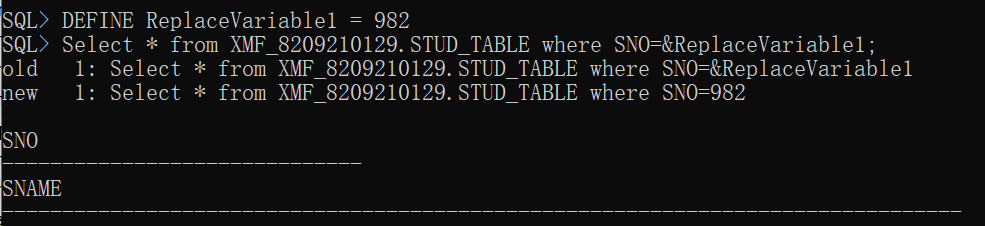
\includegraphics[width=\textwidth]{picture/代替变量案例.png}
    \captionsetup{hypcap=false}
    \captionof{figure}{代替变量案例运行结果}
    \label{fig:代替变量案例}
  \end{minipage}
\end{center}


在这里,ReplaceVariable1是一个代替变量,SQL*Plus会在执行查询之前提示用户输入ReplaceVariable1的值,并将其替换到SQL语句中。DEFINE ReplaceVariable1 = 982 用于定义SQLPlus变量。
\subsection{绑定变量}
绑定变量是在{\bfseries\kaishu 使用(或调用)PL/SQL的 环境}中创建的,而不是在PL/SQL程序的声明段中定义的。在一个PL/SQL程序块中声明的所有变量只在执行这个程序块时可以使用。而在这个程序块执行后,这些变量所使用的内存就释放了。然而,绑定变量则不同,在程序块执行后,绑定变量依然存在并允许访问。

绑定变量是在SQL语句中使用占位符(通常是冒号:后跟变量名)来代替实际的数值或表达式。在PL/SQL中,通过使用绑定变量,可以减少SQL语句的解析次数,提高性能。绑定变量在SQL语句执行时被动态绑定,而不是在每次执行时重新解析整个SQL语句。

运行演示:
\begin{center}
  \begin{minipage}{\textwidth}
    \center
    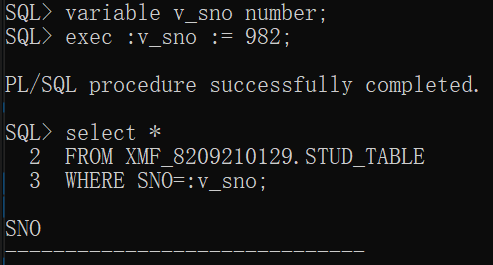
\includegraphics[width=0.5\textwidth]{picture/绑定变量效果.png}
    \captionsetup{hypcap=false}
    \captionof{figure}{绑定变量使用案例}
    \label{fig:绑定变量效果}
  \end{minipage}
\end{center}
\begin{description}
  \item[variable v\_sno number;] 定义绑定变量v\_sno
  \item[exec :v\_sno := 982] 给绑定变量赋值为982
\end{description}

\subsection{不同}

\begin{enumerate}
  \item {\bfseries\kaishu 绑定变量(Bind Variables)}
  \begin{itemize}
    \item 绑定变量是用于在SQL语句中传递数值或数据的一种机制,通过绑定变量,可以\textbf{将变量的值绑定到SQL语句中},而不是直接在SQL语句中使用硬编码的值。
    \item 这有助于提高性能,因为数据库可以缓存已编译的SQL语句,并在执行时仅替换绑定变量的值,而\textbf{不需要重新编译}整个SQL语句。
  \end{itemize}
  \item {\bfseries\kaishu 代替变量(Substitution Variables)}
  \begin{itemize}
    \item 代替变量是一种SQLPlus工具的功能,它允许在SQLPlus中使用变量,这些变量在脚本运行之前由用户手动输入,或者可以通过DEFINE命令定义。
    \item 代替变量在SQL*Plus脚本中被替换为相应的值,类似于\textbf{宏替换}。
  \end{itemize}
\end{enumerate}
\section{LOB变量}
大对象LOB是 large object的缩写,就意味着存储大量的数据,在数据库中,表中的列定义为LOB类型(如CLOB和BLOB)。利用LOB数据类型,可以在数据库中存储大量的无结构数据块(如正文、图形、声音和影像信息),其存储量可多达128T(数据量的多少取决于数据块大小)。
\subsection{LOB变量类型}
\subsubsection{CLOB数据类型(Character Large Object)}
CLOB用于在数据库中存储字节流类型的大数据对象,如演讲稿、说明书或简历等。
\subsubsection{BLOB数据类型(Binary Large Object)}
用于在数据库中存储大的二进制对象,如照片或幻灯片等。当从数据库中提取这样的数据或向数据库中插入这样的数据时,数据库并不解释这些数据。使用这些数据的外部应用程序必须自己解释这些数据。
\subsubsection{BFILE数据类型(Binary File)}
用于在数据库外的操作系统文件中存储大的二进制对象,如电影胶片等。与其他的LOB数据类型不同,BFILE数据类型是外部数据类型。BFILE类型是存储在数据库之外的,它们可能是操作系统文件。
\subsubsection{NCLOB数据类型(National Language Character Large Object)}用于在数据库中存储NCHAR类型的单字节或定长多字节的Unicode大数据对象。
\subsection{LOB变量使用}
\begin{plsql}[caption=LOB变量使用示例代码]
DECLARE
  clob_data CLOB;
  buffer VARCHAR2(32767);
  amount NUMBER;
  offset NUMBER := 1;
BEGIN
  -- 初始化 CLOB 数据
  clob_data := '这是一个CLOB示例。';
  -- 读取 CLOB 数据
  amount := DBMS_LOB.GETLENGTH(clob_data);
  DBMS_LOB.READ(clob_data, amount, offset, buffer);
  DBMS_OUTPUT.PUT_LINE(buffer);
END;
\end{plsql}

运行结果:
\begin{center}
  \begin{minipage}{\textwidth}
    \center
    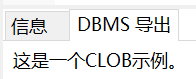
\includegraphics[width=0.3\textwidth]{picture/CLOB示例.png}
    \captionsetup{hypcap=false}
    \captionof{figure}{CLOB示例代码运行结果}
    \label{fig:CLOB示例}
  \end{minipage}
\end{center}

% 文章结束
\end{document}